\subsection{Topologia del Sistema}

La topologia del sistema è rappresentata nel seguente schema:

\begin{figure}[h]
    \centering
    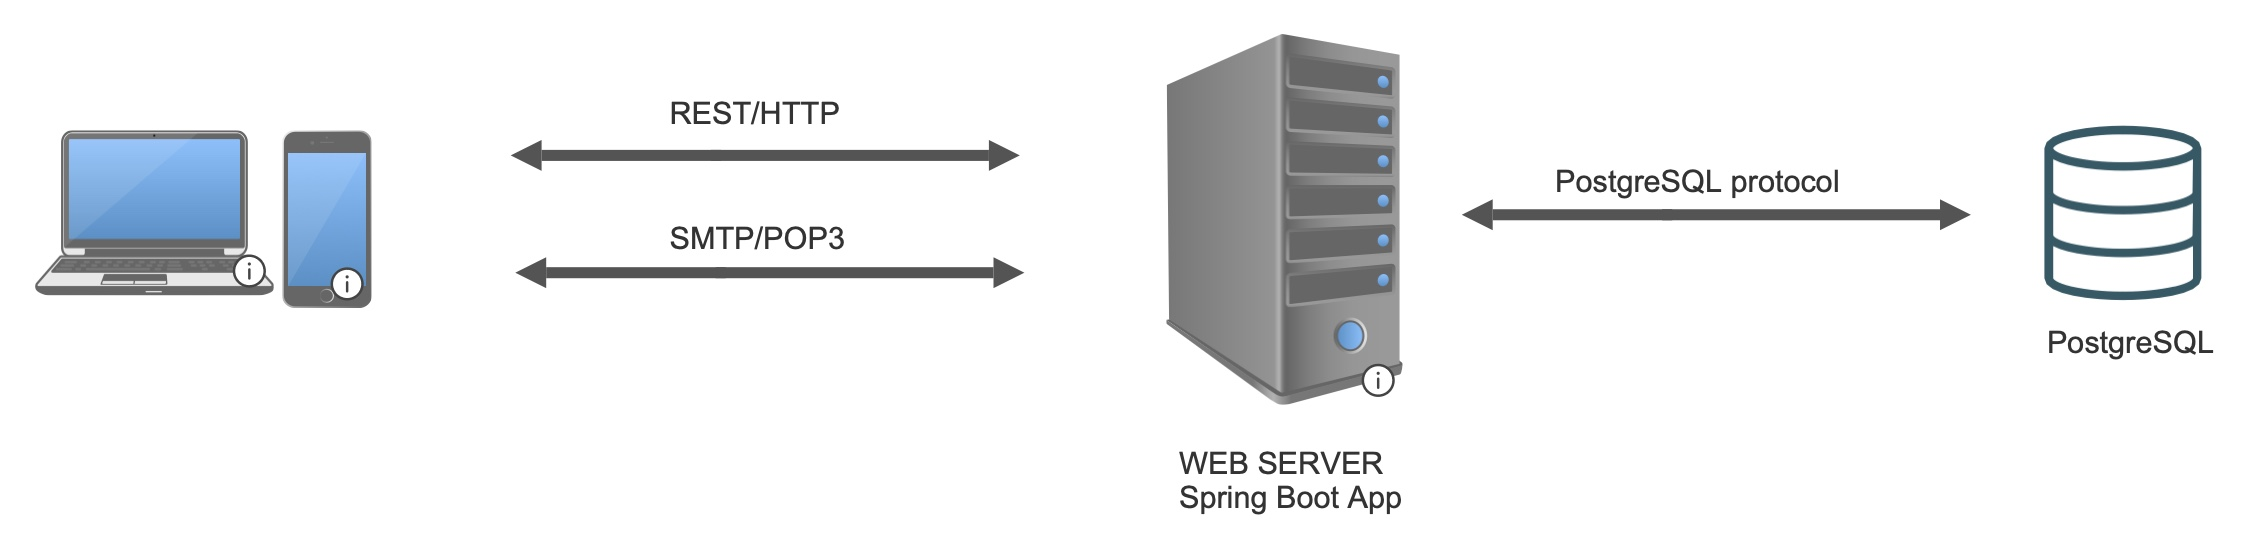
\includegraphics[scale=0.18]{images/topologia.jpg}
    \caption{Diagramma dell'architettura della webapp}
\end{figure}

Il sistema è basato su un'architettura \textbf{Client-Server} in cui i client interagiscono con un \textbf{web server} sviluppato con il framework \textbf{Spring Boot}. I client possono essere:

\begin{itemize}
    \item \textbf{Applicazione Web}: gli utenti accedono alla webapp tramite un browser, comunicando con il server attraverso \textbf{API REST/HTTP}.
    \item \textbf{Applicazione Mobile}: gli utenti possono interagire con il sistema tramite un'app mobile che utilizza \textbf{REST/HTTP} per le richieste e \textbf{SMTP/POP3} per le notifiche via email.
\end{itemize}

Il web server, sviluppato con \textbf{Spring Boot}, gestisce le richieste provenienti dai client e si interfaccia con un database \textbf{PostgreSQL} tramite il \textbf{protocollo PostgreSQL}, garantendo la persistenza dei dati.

\subsubsection{Gestione delle comunicazioni}
Il sistema sfrutta il protocollo \textbf{REST/HTTP} per lo scambio di dati in formato \textbf{JSON}, garantendo interoperabilità con diverse piattaforme. Inoltre, per le notifiche agli utenti, viene utilizzato il protocollo \textbf{SMTP/POP3}.

\subsubsection{Architettura a Microservizi}
L'architettura del sistema segue il paradigma dei \textbf{microservizi}, in cui ogni funzionalità del web server è implementata come un servizio indipendente. Questo approccio consente maggiore scalabilità, modularità e manutenibilità del sistema.